\chapter{Il Colore}
\section{Descrizione fisica}
\subsection{Definizioni}
Il colore è la traduzione da parte del nostro cervello di un fenomeno fisico. Possiamo descrivere questo fenomeno come uno spettro che assegna a ogni lunghezza (o frequenza) d'onda visibile la sua energia. Sullo spettro definiamo:
\begin{description}
	\item[Lunghezza d'onda dominante] la lunghezza d'onda della componente più energetica, è detta anche \textbf{hue}
	\item[Saturazione] il rapporto tra l'energia della hue e il valor medio dello spettro (luce bianca)
	\item[Radianza] l'energia emessa da una certa sergente (è l'integrale dello spettro)
	\item[Luminanza] energia percepita da un osservatore
	\item[Brightness] intensità della componente acromatica
	\item[Cromaticity] o \textbf{chroma} hue + saturazione
\end{description}

\section{Modelli di colore}\label{sec:color_model}
Per descrivere un colore si possono usare vari modelli che differiscono nel modo di rappresentare l'informazione, ma sono tutti equivalenti e hanno la stessa capacità espressiva Questi modelli definiscono dei volumi di colore in cui ciasun punto rappresenta un colore diverso, sono per questo detti \textbf{spazi colore}.
\subsection{Cubo RGB}
In questo modello si definisce un cubo di lato 1 avente un vertice nell'origine degli assi. Ogni asse rappresenta una componente e ogni punto all'interno del cubo sarà un colore avente un ben preciso rapporto tra le componenti. Questo modello è molto semplice e adatto a un calcolatore, ma è difficile da usare per gli umani, sono state quindi proposte alternative.
\subsection{Modelli HS*}
Questa famiglia di modelli si basano sul modo umano di rappresentare il colore e descrivono 
\begin{itemize}
	\item \textbf{Hue}: la tinta del colore
	\item \textbf{Saturazione}: quanto il colore è puro
	\item \textbf{Luminosità}: quanto ci appare brillante
\end{itemize}
Tutti i modelli HS* sono derivati applicando delle trasformazioni al cubo RGB, in particolare in tutti i modelli si ruota il cubo in modo che la diagonale che congiunge il bianco al nero sia verticale.

\begin{wrapfigure}{r}{.5\linewidth}
	\hspace{.09\linewidth}
	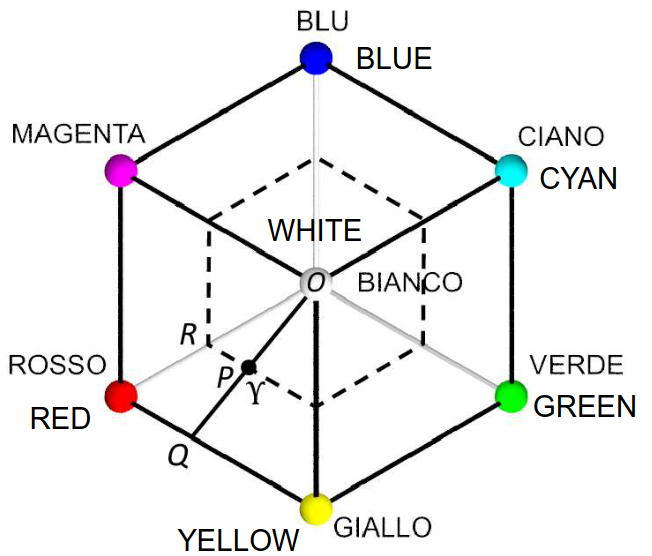
\includegraphics[width=.9\linewidth]{Picture/Cromaticity_Plane}
\end{wrapfigure}
Il piano che si ottiene guardando dall'alto i cubo ruotato è detto \textbf{chromaticity plane}. Su questo si definisce la \textbf{chroma} e la \textbf{hue} del colore $\Upsilon$
\begin{align}
	chroma(\Upsilon) &= \frac{OP}{OQ}\\
	hue(\Upsilon) &= \frac{RP}{6OR}
\end{align}

Cioè la chroma è il rapporto tra la distanza del colore dal bianco e la distanza dal bianco della tinta pura; mentre la hue è il rapporto tra la distanza dal rosso (in senso orario) e il perimetro dell'esagono.
\subsection{Spazio HSV}
In questo spazio il piano della cromaticità viene alzato fino al bianco, si rende questo esagono un cerchio e la base si trasforma in un cerchio nero, ottenendo alla fine un cilindro. Hue e croma sono definite come prima, si aggiunge il $value(\Upsilon)$ che rappresenta l'altezza sul cilindro. Si definisce poi la saturazione come:\\
\begin{minipage}{.8\linewidth}
	\vspace{-.5cm}
	\begin{equation}
		saturation(\Upsilon) = 
		\begin{cases}
			0 & if\ value(\Upsilon) = 0 \\
			\frac{chroma(\Upsilon)}{value(\Upsilon)} & otherwise
		\end{cases}
	\end{equation}
\end{minipage}
\hspace{.05\linewidth}
\begin{minipage}{.15\linewidth}
	\centering
	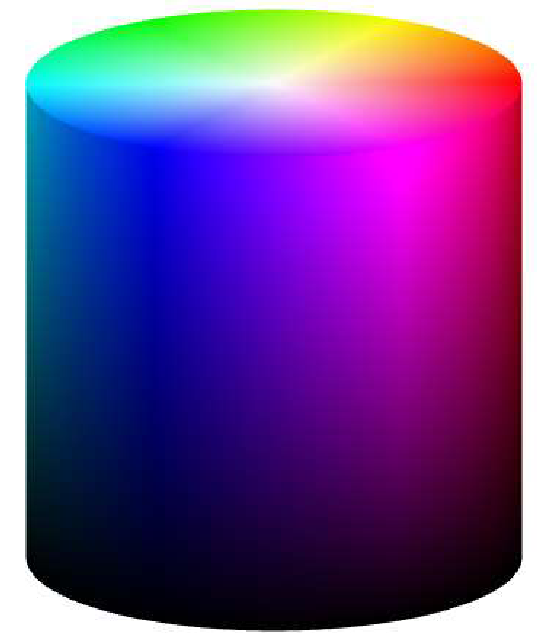
\includegraphics[width=.9\linewidth]{Picture/HSV_Space}
\end{minipage}

\subsection{Spazio HSL}
Anche in questo spazio colore si ottiene un cilindro ma il piano della cromaticità rimane al centro, mentre la faccia superiore è completamente bianca e quella inferiore completamente nera. In questo caso l'altezza sul cilindro si chiama $lightness(\Upsilon)$ (abbreviata nella formula sotto con $light$). La saturazione invece è:\\
\begin{minipage}{.8\linewidth}
	\vspace{-.5cm}
	\begin{equation}
		saturation(\Upsilon) = 
		\begin{cases}
			0 & light(\Upsilon) = 0\ \text{or}\ 1 \\
			\frac{chroma(\Upsilon)}{1 - |2\cdot light(\Upsilon) -1} & otherwise
		\end{cases}
	\end{equation}
\end{minipage}
\hspace{.05\linewidth}
\begin{minipage}{.15\linewidth}
	\centering
	\includegraphics[width=.9\linewidth, height=2cm]{Picture/HSl_Space}
\end{minipage}
\subsection{Spazio HSI}
È un modello che cerca il migliore compromesso tra comodità di rappresentazione ed efficienza sul calcolatore. Si parte sempre dal cubo ruotato, per poi normalizzarlo in modo che la diagonale sia lunga 1. In questo modello definiamo l'intensità $I$ come la somma delle componenti colorate diviso tre e la saturazione come 1 meno la componente più piccola, tutto diviso l'intensità. Con queste definizioni il modello rimane comodo per un utilizzatore e la conversione nelle componenti RGB risulta molto efficiente.

\section{Trasformazioni di colore}
\subsection{Trasformazioni in Pseudocolore}
Un immagine in scala di grigi con una profondità colore di 8 bit permette di avere 256 livelli di grigio differenti, nelle immagini mediche la profondità colore è ancora maggiore. L'occhio umano però non è sensibile a così tanti livelli di grigio, per migliorare la percezione si può trasformare una immagine monocromatica in una a falsi colori. 
\subsubsection{Intensity slicing}
\begin{wrapfigure}{r}{.4\linewidth}
	\centering
	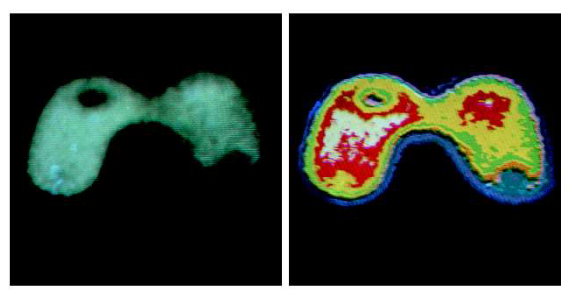
\includegraphics[width=.9\linewidth]{Picture/Pseudocolor}
\end{wrapfigure}
È una particolare trasformazione in pseudocolori che consiste nell'associare a ogni range di valori in scala di grigi un colore. In questo modo ogni pixel è colorato in base al suo livello di intensità. Come si vede dall'esempio questo metodo permette di distinguere molto meglio le varie zone dell'immagine.
\subsection{Trasformazione in falsi colori}
In questo caso si parte da un immagine a colori e si mappano i vari colori su altri colori, a esempio per evidenziare particolari dettagli. Una trasformazione di questo tipo può essere espressa come matrice di trasformazione che prende come input il vettore che contiene le componenti di colore di ciascun pixel:
\begin{equation}
	\begin{bmatrix}
		R'\\
		G'\\
		B'
	\end{bmatrix}
	= 
	\begin{bmatrix}
		c_{11} & c_{12} & c_{13} \\
		c_{21} & c_{22} & c_{23} \\
		c_{31} & c_{32} & c_{33} 
	\end{bmatrix}
	\times
	\begin{bmatrix}
		R\\
		G\\
		B
	\end{bmatrix}
\end{equation}
